% ====================================================================
% Capítulo 10: Termomayorización
% ====================================================================
\chapter{Unificación termodinámica: el preorden de termomayorización}
\label{ch:termomajorizacion}

\section{El problema de la dependencia de métrica}

Una crítica recurrente al concepto de efecto Mpemba en la literatura previa a 
2025 era la \emph{dependencia de la métrica}~\cite{burridge2016}: distintas 
funciones de distancia ---divergencia de Kullback-Leibler, distancia $L_1$, 
entropía de Shannon, distancias de Rényi--- podían dar resultados 
contradictorios sobre la presencia o ausencia del efecto en un mismo sistema.

\begin{example}[Ambigüedad métrica, Vu-Hayakawa 2025]
\label{ex:metric_ambiguity}
Sean dos distribuciones $\vb{p}_1, \vb{p}_2$ relajando al equilibrio $\pieq$. 
Es posible que $\DLone(\vb{p}_1, \pieq) > \DLone(\vb{p}_2, \pieq)$ pero 
$\DKL(\vb{p}_1, \pieq) < \DKL(\vb{p}_2, \pieq)$ en un mismo instante $t$. En 
tal caso, la métrica $L_1$ ``dice'' que $\vb{p}_2$ es más cercana al equilibrio 
y la KL dice lo contrario.
\end{example}

\noindent Esta ambigüedad puso en duda la \emph{realidad física} del efecto 
Mpemba: ¿es el cruzamiento de las curvas de relajación una característica 
genuina del sistema, o un artefacto de la métrica?

\section{La solución de Vu-Hayakawa: el preorden de termomayorización}

Tan Van Vu y Hisao Hayakawa~\cite{vuhayakawa2025} propusieron en 2025 una 
unificación matemática rigurosa basada en la teoría de \emph{termomayorización}, 
originalmente desarrollada en el contexto de la teoría de recursos termodinámicos 
cuánticos~\cite{lostaglio2022}.

\subsection{Definición del preorden}

\begin{definition}[Termomayorización]
\label{def:thermomajorization}
Sean dos distribuciones de probabilidad $\vb{p}, \vb{q}$ sobre el espacio de 
estados $\Omega = \{1, \ldots, N\}$ con energías $\{E_i\}$, y sea 
$\gamma_{i} = e^{-\beta_{b} E_{i}}/Z(\Tb)$ la distribución de Gibbs del baño. Se 
dice que $\vb{p}$ \emph{termomayoriza} a $\vb{q}$ respecto al baño $\Tb$, 
denotado $\vb{p} \succeq_{\Tb} \vb{q}$, si existe una matriz estocástica 
$\Phi$ que preserva la distribución de Gibbs ($\Phi \gamma = \gamma$) tal que 
$\Phi \vb{p} = \vb{q}$.
\end{definition}

\noindent En palabras: $\vb{p} \succeq_{\Tb} \vb{q}$ si $\vb{q}$ se puede 
obtener a partir de $\vb{p}$ aplicando una operación que respete el equilibrio 
del baño. Esto significa que $\vb{p}$ es ``más lejos del equilibrio'' que 
$\vb{q}$ en un sentido robusto, independiente de la métrica.

\subsection{Construcción explícita: la curva de Lorenz térmica}

La construcción geométrica del preorden es mediante la \emph{curva de Lorenz 
térmica}:

\begin{enumerate}
\item Calcular las razones $r_i = p_i / \gamma_i$.
\item Ordenar los índices $i$ en orden decreciente de $r_i$: 
$r_{\pi(1)} \geq r_{\pi(2)} \geq \cdots \geq r_{\pi(N)}$ (\emph{beta-ordering}).
\item Definir la curva poligonal con vértices
\begin{equation}
    (X_k, Y_k) = \left( \sum_{j=1}^{k} \gamma_{\pi(j)}, \, \sum_{j=1}^{k} p_{\pi(j)} \right), 
    \qquad k = 0, 1, \ldots, N.
\end{equation}
La curva conecta $(0,0)$ con $(1,1)$.
\end{enumerate}

\begin{theorem}[Caracterización geométrica de la termomayorización]
\label{thm:lorenz_curve}
$\vb{p} \succeq_{\Tb} \vb{q}$ si y solo si la curva de Lorenz térmica de $\vb{p}$ 
está \emph{enteramente por encima o sobre} la de $\vb{q}$ en el intervalo 
$[0, 1]$.
\end{theorem}

\begin{figure}[h]
\centering
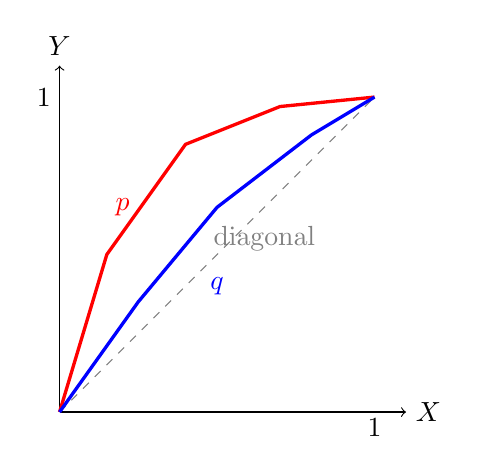
\begin{tikzpicture}[scale=4]
\draw[->] (0,0) -- (1.1,0) node[right] {$X$};
\draw[->] (0,0) -- (0,1.1) node[above] {$Y$};
\draw[gray, thin, dashed] (0,0) -- (1,1);
% curve p (above)
\draw[red, very thick] (0,0) -- (0.15, 0.5) -- (0.4, 0.85) -- (0.7, 0.97) -- (1,1);
% curve q (below)
\draw[blue, very thick] (0,0) -- (0.25, 0.35) -- (0.5, 0.65) -- (0.8, 0.88) -- (1,1);
\node[red] at (0.2, 0.65) {$\vb{p}$};
\node[blue] at (0.5, 0.4) {$\vb{q}$};
\node[gray] at (0.65, 0.55) {diagonal};
\node at (1,-0.05) {1};
\node at (-0.05,1) {1};
\end{tikzpicture}
\caption{Curvas de Lorenz térmicas. $\vb{p}$ (roja) termomayoriza a $\vb{q}$ 
(azul) porque su curva está enteramente por encima. La diagonal corresponde a 
la distribución de equilibrio $\gamma$.}
\label{fig:lorenz}
\end{figure}

\section{El teorema de equivalencia de métricas}

El resultado central de Vu-Hayakawa~\cite{vuhayakawa2025} es el siguiente 
teorema:

\begin{theorem}[Equivalencia con f-divergencias contractivas]
\label{thm:vu_hayakawa}
$\vb{p} \succeq_{\Tb} \vb{q}$ si y solo si
\begin{equation}
    D_{f}(\vb{p} \| \gamma) \geq D_{f}(\vb{q} \| \gamma) 
    \quad \text{para toda } D_{f} \text{ contractiva bajo mapas que preservan Gibbs.}
    \label{eq:vu_hayakawa}
\end{equation}
\end{theorem}

\noindent Donde una $f$-divergencia se define como
\begin{equation}
    D_{f}(\vb{p} \| \vb{q}) = \sum_{i} q_{i} f(p_{i}/q_{i}),
\end{equation}
%
con $f: \mathbb{R}_{+} \to \mathbb{R}$ convexa y $f(1) = 0$. Las clases 
incluyen:
\begin{itemize}
\item Kullback-Leibler: $f(x) = x \ln x$, $\DKL = D_{f}$.
\item Distancia $L_1$ (variación total): $f(x) = \tfrac{1}{2}\abs{x-1}$.
\item Entropías de Rényi: $f_{\alpha}(x) = (x^{\alpha} - 1)/(\alpha - 1)$ para 
$\alpha > 0$.
\item Distancia de Hellinger al cuadrado: $f(x) = (\sqrt{x} - 1)^2$.
\end{itemize}

\subsection{Demostración del teorema (esquema)}

La demostración se basa en:
\begin{enumerate}
\item Cada $f$-divergencia contractiva tiene una representación dual mediante 
una familia uniparamétrica de barreras (la $r$-divergencia).
\item La termomayorización es equivalente a que las integrales de la curva de 
Lorenz contra cualquier función monótona estén ordenadas.
\item Ambas equivalencias coinciden vía el teorema de Hardy-Littlewood-Pólya 
generalizado a la termomayorización por Ruch-Mead (1976) y refinado por 
Lostaglio (2022).
\end{enumerate}

\noindent La demostración completa en el caso clásico se da en el apéndice 
\ref{ap:thermomajorization_proofs}.

\section{Definición universal del efecto Mpemba}

Con el preorden de termomayorización, Vu-Hayakawa proponen la \emph{definición 
universal} del efecto Mpemba:

\begin{definition}[Efecto Mpemba universal, Vu-Hayakawa 2025]
\label{def:mpemba_universal}
Sean dos trayectorias de relajación $\{\vb{p}_h(t)\}, \{\vb{p}_w(t)\}$ desde 
preparaciones $\Th > \Tw > \Tb$. El \emph{efecto Mpemba universal} ocurre si 
existe $t^{\ast} > 0$ tal que
\begin{equation}
    \vb{p}_w(t^{\ast}) \succeq_{\Tb} \vb{p}_h(t^{\ast}),
\end{equation}
\emph{con desigualdad estricta} (las curvas de Lorenz no son idénticas).
\end{definition}

\noindent La virtud de esta definición es su \emph{robustez}: si el efecto está 
presente en el sentido universal, está presente \emph{simultáneamente} en 
\emph{todas} las métricas $f$-divergentes monótonas. Reciprocamente, si los 
órdenes de Lorenz se cruzan, el ``efecto Mpemba'' es ambiguo: aparece o 
desaparece según la métrica.

\section{Diagnóstico operacional: gap mínimo y máximo}

Para implementación numérica, se define el \emph{gap} signado entre curvas:
\begin{equation}
    \Delta(x; t) \equiv Y_{w}(x; t) - Y_{h}(x; t), \qquad x \in [0, 1].
\end{equation}
%
Las cantidades operacionalmente relevantes son:
\begin{itemize}
\item $\Delta_{\max}(t) = \max_{x} \Delta(x; t)$: máximo signado del exceso de 
$\vb{p}_w$ sobre $\vb{p}_h$.
\item $\Delta_{\min}(t) = \min_{x} \Delta(x; t)$.
\end{itemize}

\noindent Tres regímenes posibles:
\begin{enumerate}
\item $\Delta_{\min} \geq 0$ y $\Delta_{\max} > 0$: $\vb{p}_w \succeq_{\Tb} \vb{p}_h$ 
\emph{estricto}. Efecto Mpemba certificado para todas las métricas.
\item $\Delta_{\max} \leq 0$ y $\Delta_{\min} < 0$: $\vb{p}_h \succeq_{\Tb} \vb{p}_w$. 
La preparación caliente sigue más lejos del equilibrio.
\item $\Delta_{\max} > 0$ y $\Delta_{\min} < 0$ (las curvas se cruzan): orden 
\emph{indefinido}; el efecto es dependiente de la métrica.
\end{enumerate}

\section{Aplicación al sistema markoviano de tres estados}

Aplicando el diagnóstico de termomayorización al sistema de tres estados de 
Lu-Raz~\cite{lu2017}, se obtiene la trayectoria temporal de 
$(\Delta_{\max}, \Delta_{\min})$ mostrada en \cref{fig:thermo_diagnostic}.

\begin{itemize}
\item En $t = 0$: $\Delta_{\max} \approx 0.084$, $\Delta_{\min} = 0$. La 
preparación caliente domina (es estrictamente más lejos del equilibrio).
\item A $t \approx 8$: $\Delta_{\min}$ cruza cero hacia valores negativos. 
\emph{El orden se invierte: la preparación fría es ahora más lejos del 
equilibrio.}
\item Para $t > 8$: $\Delta_{\min} < 0$ persistentemente, certificando el 
efecto Mpemba universal.
\end{itemize}

\noindent Es notable que la \emph{certificación termomayorización} ocurre a 
$t \approx 8$, mientras que el \emph{cruzamiento de la métrica entrópica} 
ocurre a $t \approx 22.4$. La razón: la termomayorización es una condición 
\emph{más exigente} (todas las métricas simultáneamente), por lo que su 
detección en términos de pérdida de dominancia ocurre más temprano.

\begin{figure}[h]
\centering
\fbox{\parbox{0.85\textwidth}{\centering \emph{Figura: $\Delta_{\max}(t)$ y 
$\Delta_{\min}(t)$ para el sistema de Lu-Raz. La inversión de signo a $t \approx 8$ 
certifica el efecto Mpemba universal.}\\[2cm]
[Archivo: results/markovian/thermomajorization\_diagnostic.csv]}}
\caption{Diagnóstico de termomayorización aplicado al sistema markoviano de 
tres estados.}
\label{fig:thermo_diagnostic}
\end{figure}

\section{Extensión a recursos correlacionados}

Vu y Hayakawa~\cite{vuhayakawa2025_resources} extendieron el formalismo a 
sistemas con \emph{correlaciones no locales}, demostrando que la 
termomayorización proporciona los \emph{límites independientes de la dinámica} 
para el enfriamiento térmico. En particular, para un sistema $A \otimes B$ con 
estado conjunto $\rho_{AB}$:
\begin{equation}
    T_{h}^{\max}(\Tc) = \sup \{ T : \rho_{AB}(T) \succeq_{\Tb} \rho_{AB}(\Tc) \},
\end{equation}
%
da la temperatura efectiva máxima ante la cual un estado correlacionado frío 
permanece más alejado del equilibrio que un estado caliente Gibbsiano puro.

\section{Implementación del módulo}

El módulo \texttt{mpemba\_thermomajorization} de \texttt{Mpemba-X v2} implementa 
en \texttt{core/thermomajorization.hpp}:

\begin{lstlisting}[language=C++, caption={Construcción de la curva de Lorenz térmica}, label={lst:thermomaj_cpp}]
ThermomajorizationCurve build_thermomaj_curve(
    const std::vector<double>& p,
    const std::vector<double>& energies,
    double T_b) 
{
    int n = p.size();
    // Calcular distribución de Gibbs
    std::vector<double> gamma(n);
    double Z = 0.0;
    for (int i = 0; i < n; ++i) {
        gamma[i] = std::exp(-energies[i] / T_b);
        Z += gamma[i];
    }
    for (auto& g : gamma) g /= Z;
    
    // Beta-ordering: ordenar por p_i / gamma_i descendente
    std::vector<int> order(n);
    std::iota(order.begin(), order.end(), 0);
    std::sort(order.begin(), order.end(),
        [&](int a, int b) { return p[a]/gamma[a] > p[b]/gamma[b]; });
    
    // Construir vertices acumulando
    ThermomajorizationCurve c;
    c.X.push_back(0.0); c.Y.push_back(0.0);
    double sx = 0, sy = 0;
    for (int k : order) {
        sx += gamma[k]; sy += p[k];
        c.X.push_back(sx); c.Y.push_back(sy);
    }
    return c;
}
\end{lstlisting}
%
\noindent La comparación de dos curvas se realiza por interpolación lineal en 
una grilla fina de $4096$ puntos en $[0, 1]$.
